\documentclass[utf8,compress]{beamer}
\usepackage[utf8]{inputenc}
\usepackage[T1]{fontenc}
\usepackage{irbookslide}
\usepackage{irilmenau2}

\title{Simulacija sistema i dizajn programa}
\subtitle{\tiny{Slajdovi za predmet Osnove programiranja}}
\subject{Osnove programiranja}
\institute{Katedra za informatiku, Fakultet tehničkih nauka, Novi Sad}
\date{2011.}

\begin{document}

\frame{\titlepage}

\frame{
  \frametitle{Ciljevi}
  \begin{itemize}
    \item potencijalne primene simulacije kao sredstva za rešavanje realnih problema
    \item pseudoslučajni brojevi i njihova primena u Monte Carlo simulacijama
    \item primena top-down i spiralnih tehnika u pisanju složenih programa
    \item jedinično testiranje i otkrivanje grešaka u složenim programima
  \end{itemize}
}

\section[Simulacija]{Simulacija}

\frame{
  \frametitle{Simuliranje racquetballa}
  \begin{itemize}
    \item \myblue{simulacijom} modelujemo realne procese
    \item na taj način možemo dobiti informacije koje bismo teško dobili na drugačiji način
    \item primene simulacije: vremenska prognoza, dizajn letelica, specijalni filmski efekti, itd.
  \end{itemize}
}

\begin{frame}
  \frametitle{Problem koji simuliramo}
  \begin{itemize}
    \item Žika često igra racquetball sa protivnicima koji su malo bolji od njega
    \item Žika obično gubi mečeve!
    \item zar ne bi igrači koji su \textbf{malo} bolji trebali da pobeđuju \textbf{malo} češće?
    \item simulacijom možemo ustanoviti da li male razlike u sposobnostima uzrokuju velike razlike u rezultatima
  \end{itemize}
\end{frame}

\begin{frame}
  \frametitle{Analiza i specifikacija}
  \begin{itemize}
    \item racquetball igraju 2 igrača na terenu unutar 4 zida
    \item jedan igrač počinje igru \textbf{servisom}
    \item igrači se smenjuju udarajući lopticu reketom -- \textbf{reli}
    \item reli se završava kada prvi igrač ne uspe da vrati lopticu u igru
  \end{itemize}
\end{frame}

\begin{frame}
  \frametitle{Analiza i specifikacija $_2$}
  \begin{itemize}
    \item ako je pogrešio igrač koji je servirao, servis preuzima drugi igrač
    \item ako je pogrešio igrač koji nije servirao, igrač koji je servirao dobija poen
    \item igrači mogu osvajati poene samo na svoj servis!
    \item prvi igrač koji osvoji 15 poena je pobednik
  \end{itemize}
\end{frame}

\begin{frame}
  \frametitle{Analiza i specifikacija $_3$}
  \begin{itemize}
    \item u našoj simulaciji sposobnost igrača se izražava kao verovatnoća da će igrač osvojiti reli na svoj servis
    \item primer: igrač sa verovatnoćom 0.6 će osvojiti 60\% relija na svoj servis
    \item program će omogućiti unos verovatnoće za oba igrača i zatim simulirati više partija
    \item na kraju će ispisati rezultate simulacije
  \end{itemize}
\end{frame}

\begin{frame}
  \frametitle{Ulazni podaci}
  \begin{itemize}
    \item verovatnoće osvajanja poena za igrače A i B; 
    \item broj partija koje će odigrati A i B
  \end{itemize}
\end{frame}

\begin{frame}
  \frametitle{Izlazni podaci}
  \begin{itemize}
    \item broj odigranih partija
    \item broj pobeda i procenat pobeda za igrače A i B
  \end{itemize}
\end{frame}

\begin{frame}
  \frametitle{Napomene}
  \begin{itemize}
    \item pretpostavljamo da su svi ulazni podaci ispravne numeričke vrednosti
    \item u svakoj simuliranoj partiji igrač A počinje prvi
  \end{itemize}
\end{frame}

\section[Random]{Pseudoslučajni brojevi}

\begin{frame}
  \frametitle{Verovatnoća}
  \begin{itemize}
    \item kada kažemo da igrač A pobeđuje u 50\% relija, to ne znači da pobeđuje \textbf{fiksno} svaki drugi put
    \item više liči na bacanje novčića
    \item u proseku, u pola slučajeva će pasti glava, a u drugih pola će pasti pismo
    \item rezultat jednog bacanja novčića ne utiče na sledeće bacanje
    \item može se desiti da 5 puta uzastopno padne glava
  \end{itemize}
\end{frame}

\begin{frame}
  \frametitle{Verovatnoća}
  \begin{itemize}
    \item veliki broj simulacija dovešće do toga da se događaji pojavljuju sa određenom \myblue{verovatnoćom}
    \item simulacije zasnovane na verovatnoći zovu se \myblue{Monte Carlo} simulacije
  \end{itemize}
\end{frame}

\begin{frame}
  \frametitle{Slučajni i pseudoslučajni brojevi}
  \begin{itemize}
    \item niz \myblue{slučajnih} brojeva: ne može se ustanoviti pravilo za određivanje narednog broja na osnovu prethodnog
    \item \myblue{pseudoslučajni} brojevi su nastali na osnovu preciznog pravila, ali čoveku \textbf{izgledaju} kao slučajni brojevi
    \item program \texttt{chaos.py} sa prvih predavanja: brojevi izgledaju nasumični, iako su izračunati po preciznoj formuli
  \end{itemize}
\end{frame}

\begin{frame}
  \frametitle{Generisanje pseudoslučajnih brojeva}
  \begin{itemize}
    \item generator pseudoslučajnih brojeva funkcioniše na sličan način
    \item počinje od inicijalne (\myblue{seed}) vrednosti
    \item na osnovu nje se izračuna ,,slučajan`` broj
    \item kada se zatraži novi broj, prethodni broj se koristi u izračunavanju
  \end{itemize}
\end{frame}

\begin{frame}
  \frametitle{Generisanje pseudoslučajnih brojeva $_2$}
  \begin{itemize}
    \item niz brojeva izgleda nasumično
    \item ako pokrenemo generator sa istim \textbf{seed}-om dobićemo isti niz ,,slučajnih`` brojeva
    \item Python ima modul koji sadrži više funkcija za rad sa pseudoslučajnim brojevima
    \item ove funkcije izračunavaju \textbf{seed} na osnovu sistemskog datuma i vremena
    \item svaki put kada se pokrene, funkcija proizvodi različit niz brojeva
  \end{itemize}
\end{frame}

\begin{frame}
  \frametitle{Funkcija \texttt{randrange}}
  \begin{itemize}
    \item funkcija \texttt{randrange} vraća pseudoslučajan \texttt{int} iz datog opsega
    \item sintaksa je slična funkciji \texttt{range}
    \item \texttt{randrange(1, 6)} \\
      vraća ,,slučajno`` izabran broj iz \texttt{[1,2,3,4,5]}
    \item \texttt{randrange(5, 105, 5)} \\
      vraća ,,slučajno`` izabran broj iz \texttt{[5,10,15,20,...,100]}
    \item gornja granica za \texttt{randrange} ne ulazi u moguće vrednosti
  \end{itemize}
\end{frame}

\begin{frame}[fragile,shrink=5]
  \frametitle{Funkcija \texttt{randrange} $_2$}
  \begin{itemize}
    \item svaki poziv \texttt{randrange} proizvodi jedan pseudoslučajan \texttt{int}
  \end{itemize}
\begin{verbatim}
>>> from random import randrange
>>> randrange(1,6)
5
>>> randrange(1,6)
3
>>> randrange(1,6)
2
>>> randrange(1,6)
5
>>> randrange(1,6)
5
>>> randrange(1,6)
5
>>> randrange(1,6)
4
\end{verbatim}
\end{frame}

\begin{frame}
  \frametitle{Funkcija \texttt{randrange} $_3$}
  \begin{itemize}
    \item desilo se da se broj 5 pojavi više puta
    \item na velikom broju pokušaja dobićemo \myblue{uniformnu raspodelu}
    \item tj. sve vrednosti će se pojaviti otprilike jednak broj puta
  \end{itemize}
\end{frame}

\begin{frame}
  \frametitle{Funkcija \texttt{random}}
  \begin{itemize}
    \item funkcija \texttt{random} vraća pseudoslučajne \texttt{float} brojeve
    \item \texttt{random} nema parametre
    \item uvek vraća broj iz opsega $[0,1)$
  \end{itemize}
\end{frame}

\begin{frame}[fragile]
  \frametitle{Funkcija \texttt{random} $_2$}
\begin{verbatim}
>>> from random import random
>>> random()
0.79432800912898816
>>> random()
0.00049858619405451776
>>> random()
0.1341231400816878
>>> random()
0.98724554535361653
>>> random()
0.21429424175032197
>>> random()
0.23903583712127141
>>> random()
0.72918328843408919
\end{verbatim}
\end{frame}

\begin{frame}[fragile]
  \frametitle{\texttt{random} i racquetball}
  \begin{itemize}
    \item simulacija racquetball partije koristi funkciju \texttt{random}
    \item ako je verovatnoća osvajanja poena za igrača 70\% odnosno 0.7
  \end{itemize}
\begin{verbatim}
if <igrač dobije na svoj servis>:
    score = score + 1
\end{verbatim}
  \begin{itemize}
    \item treba nam izraz koji vraća \texttt{True} u 70\% slučajeva
  \end{itemize}
\end{frame}

\begin{frame}
  \frametitle{\texttt{random} i racquetball $_2$}
  \begin{itemize}
    \item recimo da generišemo broj iz $[0,1)$
    \item 70\% tog intervala se nalazi levo od tačke 0.7
    \item u 70\% slučajeva broj će biti manji od 0.7
    \item u preostalih 30\% slučajeva će biti $\geq 0.7$
    \item = ide na gornji kraj intervala jer generator može da proizvede 0 ali ne i 1
  \end{itemize}
\end{frame}

\begin{frame}[fragile]
  \frametitle{\texttt{random} i racquetball $_3$}
  \begin{itemize}
    \item ako \texttt{prob} predstavlja verovatnoću za igrača
    \item uslov \texttt{random() < prob} će biti zadovoljen sa traženom verovatnoćom
  \end{itemize}
\begin{verbatim}
if random() < prob:
    score = score + 1
\end{verbatim}
\end{frame}

\section[Top-down]{Top-down dizajn}

\begin{frame}
  \frametitle{Top-down dizajn}
  \begin{itemize}
    \item \myblue{top-down dizajn} predstavlja način za rešavanje problema
    \item složen problem se predstavi kao kombinacija jednostavnijih, manjih problema
    \item ovaj princip ponavljamo dok ne dođemo do problema koji su trivijalni za rešavanje
    \item rešenja malih problema zajedno čine rešenje velikog problema
  \end{itemize}
\end{frame}

\begin{frame}[fragile]
  \frametitle{Šablon ulaz-obrada-izlaz}
  \begin{itemize}
    \item programi često koriste šablon \myblue{ulaz-obrada-izlaz}
    \item algoritam za simulaciju racquetball-a:
  \end{itemize}
\begin{verbatim}
ispiši uvodni tekst
unesi podatke: probA, probB, n
simuliraj n partija korišćenjem probA i probB
ispiši rezultate simulacije
\end{verbatim}
\end{frame}

\begin{frame}
  \frametitle{Top-down dizajn}
  \begin{itemize}
    \item da li je ovo rešenje suviše apstraktno? 
    \item sve što ne umemo da napravimo ignorisaćemo na trenutak
    \item pretpostavimo da su sve komponente koje nam trebaju da implementiramo algoritam već napravljene
    \item naš zadatak je tada jednostavan
  \end{itemize}
\end{frame}

\begin{frame}
  \frametitle{Prvi korak}
  \begin{itemize}
    \item prvo ispisujemo uvodni tekst
    \item ovo je lako, i nećemo da gubimo vreme na to \\ \ \\
      \texttt{printIntro()} \\ \ \\
    \item pretpostavljamo da postoji funkcija printIntro() koja radi baš ono što nam treba!
  \end{itemize}
\end{frame}

\begin{frame}
  \frametitle{Drugi korak}
  \begin{itemize}
    \item u drugom koraku unosimo podatke
    \item i ovo je lako
    \item recimo da postoji funkcija \texttt{getInputs} napravljena za ovaj zadatak \\ \ \\
      \texttt{printIntro()} \\
      \texttt{probA, probB, n = getInputs()}
  \end{itemize}
\end{frame}

\begin{frame}[fragile]
  \frametitle{Treći korak}
  \begin{itemize}
    \item treći korak je simulacija $n$ partija
    \item recimo da postoji funkcija \texttt{simGames} za ovaj zadatak
    \item koji ulazni podaci su njoj potrebni?
    \begin{itemize}
      \item \texttt{probA}, \texttt{probB}, \texttt{n}
    \end{itemize}
    \item koje rezultate ćemo dobiti od funkcije?
    \begin{itemize}
      \item broj partija koje je dobio A
      \item broj partija koje je dobio B
    \end{itemize}
  \end{itemize}
\begin{verbatim}
printIntro()
probA, probB, n = getInputs()
winsA, winsB = simGames(n, probA, probB)
\end{verbatim}
\end{frame}

\begin{frame}[fragile]
  \frametitle{Četrvrti korak}
  \begin{itemize}
    \item četvtrti korak je ispis rezultata simulacije
    \item recimo da postoji funkcija printSummary koja obavlja taj posao
    \item koji ulazni podaci su njoj potrebni?
    \begin{itemize}
      \item \texttt{winsA}, \texttt{winsB}
    \end{itemize}
  \end{itemize}
\begin{verbatim}
printIntro()
probA, probB, n = getInputs()
winsA, winsB = simGames(n, probA, probB)
printSummary(winsA, winsB)
\end{verbatim}
\end{frame}

\begin{frame}[fragile]
  \frametitle{Kompletan program}
\begin{verbatim}
def main():
    printIntro()
    probA, probB, n = getInputs()
    winsA, winsB = simGames(n, probA, probB)
    printSummary(winsA, winsB)

main()
\end{verbatim}
\end{frame}

\begin{frame}
  \frametitle{Razdvajanje zaduženja}
  \begin{itemize}
    \item početni problem je dekomponovan na 4 podproblema
    \begin{itemize}
      \item \texttt{printIntro}
      \item \texttt{getInputs}
      \item \texttt{simGames}
      \item \texttt{printSummary}
    \end{itemize}
    \item naziv, parametri i rezultat svake funkcije su već određeni
    \item to čini \myblue{signaturu} ili \myblue{interfejs} funkcije
    \begin{itemize}
      \item preko parametara i rezultata funkcija ,,komunicira sa spoljašnjim svetom``
    \end{itemize}
  \end{itemize}
\end{frame}

\begin{frame}
  \frametitle{Razdvajanje zaduženja $_2$}
  \begin{itemize}
    \item signature svih funkcija nam omogućavaju da nezavisno (paralelno) rešavamo te probleme
    \item kako radi \texttt{simGames} nije važno u funkciji \texttt{main}
    \item važno je samo da prima dogovorene parametre i vraća dogovoreni rezultat
  \end{itemize}
\end{frame}

\begin{frame}
  \frametitle{Razdvajanje zaduženja $_3$}
  \begin{itemize}
    \item \myblue{strukturu} našeg programa -- tj. \myblue{hijerarhiju} možemo prikazati grafički
    \item svaka funkcija je pravougaonik
    \item linija između pravougaonika označava da funkcija iznad poziva (koristi) funkciju ispod
    \item strelice označavaju prenos podataka
  \end{itemize}
\end{frame}

\begin{frame}
  \frametitle{Razdvajanje zaduženja $_4$}
  \begin{center}
    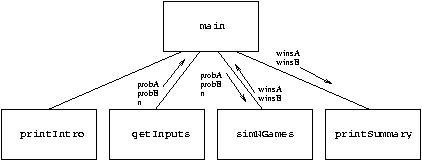
\includegraphics[width=10cm]{pic22}
  \end{center}
\end{frame}

\begin{frame}
  \frametitle{Razdvajanje zaduženja $_5$}
  \begin{itemize}
    \item na svakom nivou dizajna interfejs nam govori koji detalji sa nižeg nivoa su bitni
    \item proces određivanja bitnih osobina i ignorisanje drugih detalja zove se \myblue{apstrakcija}
    \item top-down dizajn je postupak otkrivanja korisnih apstrakcija
  \end{itemize}
\end{frame}

\begin{frame}[fragile,shrink=15]
  \frametitle{Dizajn na drugom nivou: \texttt{printIntro}}
  \begin{itemize}
    \item ponavljamo top-down pristup za svaki od podproblema koje smo već definisali
    \item funkcija \texttt{printIntro} treba da ispiše uvodnu poruku
  \end{itemize}
\begin{verbatim}
def printIntro():
    print("Ovaj program simulira racquetball partije između igrača")
    print('zvanih "A" i "B".  Sposobnost svakog igrača je određena')
    print("verovatnoćom (broj između 0 i 1) da igrač osvoji poen")
    print("na svoj servis. Igrač A uvek servira prvi.\n")
\end{verbatim}
  \begin{itemize}
    \item u drugoj liniji string je dat u jednostrukim navodnicima zato što želimo da ispišemo dvostruke navodnike
    \item nema novih funkcija $\rightarrow$ nema novih dijagrama
  \end{itemize}
\end{frame}

\begin{frame}[fragile,shrink=15]
  \frametitle{Dizajn na drugom nivou: \texttt{getInputs}}
  \begin{itemize}
    \item funkcija \texttt{getInputs} unosimo tri broja koja vraćamo kao rezultat funkcije
  \end{itemize}
\begin{verbatim}
def getInputs():
    a = eval(input("Verovatnoća da A osvoji poen na servis >> "))
    b = eval(input("Verovatnoća da B osvoji poen na servis >> "))
    n = eval(input("Broj partija za simulaciju >> "))
    return a, b, n
\end{verbatim}
\end{frame}

\begin{frame}[fragile]
  \frametitle{Dizajn na drugom nivou: \texttt{simGames}}
  \begin{itemize}
    \item funkcija \texttt{simGames} simulira $n$ partija i prati ukupan broj pobeda igrača
    \item ,,simulira $n$ partija`` zvuči kao petlja
    \item ,,prati ukupan broj`` liči na akumulator
  \end{itemize}
\begin{verbatim}
inicijalizuj winsA i winsB na 0
ponovi n puta
    simuliraj partiju
    if pobedio igrač A:
        inkrementiraj winsA
    else:
        inkrementiraj winsB
\end{verbatim}
\end{frame}

\begin{frame}[fragile]
  \frametitle{Dizajn na drugom nivou: \texttt{simGames} $_2$}
  \begin{itemize}
    \item već imamo signaturu funkcije \texttt{simGames}
  \end{itemize}
\begin{verbatim}
def simNGames(n, probA, probB):
    # simulira n racquetball partija između igrača A i B
    # vraća broj pobeda A, broj pobeda B
\end{verbatim}
  \begin{itemize}
    \item početak je lak:
  \end{itemize}
\begin{verbatim}
def simNGames(n, probA, probB):
    # simulira n racquetball partija između igrača A i B
    # vraća broj pobeda A, broj pobeda B
    winsA = 0
    winsB = 0
    for i in range(n):
\end{verbatim}
\end{frame}

\begin{frame}[fragile]
  \frametitle{Dizajn na drugom nivou: \texttt{simGames} $_3$}
  \begin{itemize}
    \item sledeći zadatak je simulacija jedne partije
    \item nismo sigurni kako to uraditi -- ostavimo to za kasnije!
    \item recimo da postoji funkcija \texttt{simOneGame}
    \item ulazi za \texttt{simOneGame} su verovatnoće za igrače A i B
    \item šta je izlaz? -- podatak ko je dobio partiju
    \item najlakše je preneti konačni rezultat (npr 15:11)
    \item pobednik je onaj sa više poena, njegov akumulator inkrementiramo
  \end{itemize}
\end{frame}

\begin{frame}[fragile]
  \frametitle{Dizajn na drugom nivou: \texttt{simGames} $_4$}
\begin{verbatim}
def simNGames(n, probA, probB):
    # simulira n racquetball partija između igrača A i B
    # vraća broj pobeda A, broj pobeda B
    winsA = winsB = 0
    for i in range(n):
        scoreA, scoreB = simOneGame(probA, probB)
        if scoreA > scoreB:
            winsA = winsA + 1
        else:
            winsB = winsB + 1
    return winsA, winsB
\end{verbatim}
\end{frame}

\begin{frame}[fragile]
  \frametitle{Dizajn na drugom nivou: \texttt{simGames} $_5$}
  \begin{center}
    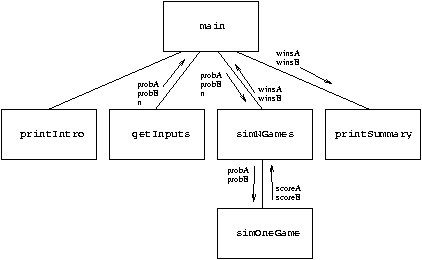
\includegraphics[width=10cm]{pic23}
  \end{center}
\end{frame}

\begin{frame}[fragile]
  \frametitle{Dizajn na trećem nivou: \texttt{simOneGame}}
\begin{itemize}
  \item igrači igraju relije dok jedan ne pobedi
  \item liči na beskonačnu petlju -- ne znamo unapred koliko će relija trajati partija
  \item treba da pamtimo rezultat -- dva akumulatora
  \item treba da pamtimo i ko servira -- string koji uzima vrednosti \\ \texttt{"A"} i \texttt{"B"}
\end{itemize}
\end{frame}

\begin{frame}[fragile]
  \frametitle{Dizajn na trećem nivou: \texttt{simOneGame} $_2$}
\begin{verbatim}
def simOneGame(probA, probB):
    scoreA = 0
    scoreB = 0
    serving = "A"
    while <uslov>:
\end{verbatim}
\begin{itemize}
  \item šta će biti \texttt{uslov}?
  \item neka prosledimo rezultat(e) funkciji koja vraća \texttt{True} ako je partija gotova
\end{itemize}
\end{frame}

\begin{frame}
  \frametitle{Dizajn na trećem nivou: \texttt{simOneGame} $_3$}
\begin{center}
  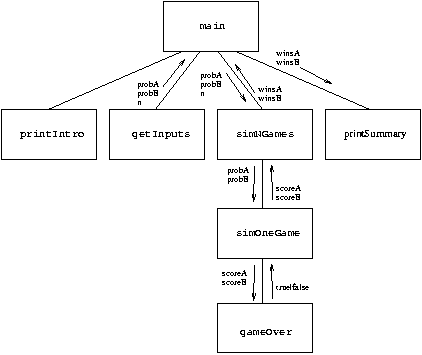
\includegraphics[width=9cm]{pic24}
\end{center}
\end{frame}

\begin{frame}[fragile]
  \frametitle{Dizajn na trećem nivou: \texttt{simOneGame} $_4$}
\begin{itemize}
  \item unutar \texttt{while} petlje treba da obradimo jedan servis
  \item poredićemo slučajan broj sa verovatnoćom igrača koji servira (\texttt{probA} ili \texttt{probB})
  \item igrača koji servira pamtimo u promenljivoj \texttt{serving}
\end{itemize}
\end{frame}

\begin{frame}[fragile]
  \frametitle{Dizajn na trećem nivou: \texttt{simOneGame} $_5$}
\begin{itemize}
  \item ako servira igrač A onda koristimo \texttt{probA}, 
  \item zavisno od rezultata ili povećamo poene za A ili servis preuzima B
\end{itemize}
\begin{verbatim}
if serving == "A":
    if random() < probA:
        scoreA = scoreA + 1
    else:
        serving = "B"
\end{verbatim}
\end{frame}

\begin{frame}[fragile]
  \frametitle{Dizajn na trećem nivou: \texttt{simOneGame} $_6$}
\begin{itemize}
  \item ako servira B, radimo isto kao i u prethodnom slučaju, samo sa zamenjenim ulogama
\end{itemize}
\begin{verbatim}
if serving == "A":
    if random() < probA:
        scoreA = scoreA + 1
    else:
        serving = "B“
else:
    if random() < probB:
        scoreB = scoreB + 1
    else:
        serving = "A"
\end{verbatim}
\end{frame}

\begin{frame}[fragile,shrink=5]
  \frametitle{Cela funkcija \texttt{simOneGame}}
\begin{verbatim}
def simOneGame(probA, probB):
    serving = "A"
    scoreA = 0
    scoreB = 0
    while not gameOver(scoreA, scoreB):
        if serving == "A":
            if random() < probA:
                scoreA = scoreA + 1
             else:
                serving = "B"
        else:
            if random() < probB:
                scoreB = scoreB + 1
            else:
                serving = "A"
    return scoreA, scoreB
\end{verbatim}
\end{frame}

\begin{frame}[fragile]
  \frametitle{Dizajn na četvrtom nivou: \texttt{gameOver}}
\begin{itemize}
  \item za sada imamo signaturu funkcije \texttt{gameOver}
\end{itemize}
\begin{verbatim}
def gameOver(a,b):
    # a i b su poeni igrača
    # vraća True ako je partija gotova, inače vraća False
\end{verbatim}
\begin{itemize}
  \item igra je gotova kada bilo koji igrač osvoji 15 poena:
\end{itemize}
\begin{verbatim}
a == 15 or b == 15
\end{verbatim}
\end{frame}

\begin{frame}[fragile]
  \frametitle{Cela funkcija \texttt{gameOver}}
\begin{verbatim}
def gameOver(a,b):
    # a i b su poeni igrača
    # vraća True ako je partija gotova, inače vraća False
    return a == 15 or b == 15
\end{verbatim}
\end{frame}

\begin{frame}[fragile]
  \frametitle{Cela funkcija \texttt{printSummary}}
\begin{verbatim}
def printSummary(winsA, winsB):
    # Ispisuje rezultate simulacije
    n = winsA + winsB
    print "\nSimulirano partija:", n
    print "Pobede A: {0} ({1:0.1%})".format(winsA, winsA/n)
    print "Pobede B: {0} ({1:0.1%})".format(winsB, winsB/n)
\end{verbatim}
\end{frame}

\begin{frame}
  \frametitle{Rezime top-down pristupa}
\begin{itemize}
  \item počeli smo sa najvišeg nivoa strukture našeg programa
  \item na svakom nivou počeli smo uopštenim algoritmom i prevodili ga u precizan kod
  \item ,,rafinacija korak-po-korak`` (step-wise refinement)
\end{itemize}
\end{frame}

\begin{frame}
  \frametitle{Rezime top-down pristupa $_2$}
\begin{itemize}
  \item[1] izrazi algoritam kao seriju manjih problema
  \item[2] definiši interfejs (signaturu) za svaki od manjih problema
  \item[3] opiši algoritam u smislu interfejsa prema manjim problemima
  \item[4] ponovi postupak za svaki manji problem
\end{itemize}
\end{frame}

\begin{frame}
  \frametitle{Bottom-up implementacija}
\begin{itemize}
  \item iako smo bili pažljivi sa dizajnom, nema garancija da nismo napravili neke greške
  \item implementaciju je najbolje praviti u malim delovima (koracima)
\end{itemize}
\end{frame}

\section[Testiranje]{Jedinično testiranje}

\begin{frame}
  \frametitle{Testiranje programa}
\begin{itemize}
  \item sistematično testiranje već od iole većeg programa:
  \item počnemo sa testiranjem na najnižem nivou strukture
  \item testiramo komponentu čim je završimo
  \item ne odlažemo testiranje za kasnije! \\ \ \\
  \item možemo \texttt{import}-ovati naš program i pozivati njegove funkcije da proverimo da li rade ispravno
\end{itemize}
\end{frame}

\begin{frame}[fragile]
  \frametitle{Primer testiranja}
\begin{itemize}
  \item možemo početi od funkcije \texttt{gameOver}
\end{itemize}
\begin{verbatim}
>>> import rball
>>> rball.gameOver(0,0)
False
>>> rball.gameOver(5,10)
False
>>> rball.gameOver(15,3)
True
>>> rball.gameOver(3,15)
True
\end{verbatim}
\end{frame}

\begin{frame}
  \frametitle{Testiranje funkcije \texttt{gameOver}}
\begin{itemize}
  \item pokrili smo sve bitne slučajeve
  \item sa 0,0 simuliramo prvi poziv ove funkcije
  \item drugi test simulira stanje u sredini partije
  \item poslednja dva testa proveravaju pobedu oba igrača
\end{itemize}
\end{frame}

\begin{frame}[fragile,shrink=10]
  \frametitle{Testiranje funkcije \texttt{simOneGame}}
\begin{itemize}
  \item sada možemo preći na testiranje funkcije \texttt{simOneGame}
\end{itemize}
\begin{verbatim}
>>> simOneGame(.5, .5)
(11, 15)
>>> simOneGame(.5, .5)
(13, 15)
>>> simOneGame(.3, .3)
(11, 15)
>>> simOneGame(.3, .3)
(15, 4)
>>> simOneGame(.4, .9)
(2, 15)
>>> simOneGame(.4, .9)
(1, 15)
>>> simOneGame(.9, .4)
(15, 0)
>>> simOneGame(.9, .4)
(15, 0)
>>> simOneGame(.4, .6)
(10, 15)
>>> simOneGame(.4, .6)
(9, 15)
\end{verbatim}
\end{frame}

\begin{frame}
  \frametitle{Testiranje funkcije \texttt{simOneGame} $_2$}
\begin{itemize}
  \item kada su verovatnoće jednake, broj poena je ,,blizu``
  \item kada su verovatnoće značajno različite, rezultat je ,,čišćenje sa terena``
\end{itemize}
\end{frame}

\begin{frame}
  \frametitle{Jedinično testiranje}
\begin{itemize}
  \item testiranje svake komponente programa -- \myblue{jedinice} -- na ovaj način zovemo \myblue{jedinično testiranje}
  \item testiranje svake funkcije nezavisno olakšava pronalaženje grešaka
  \item pojednostavljuje testiranje celog programa
\end{itemize}
\end{frame}

\begin{frame}
  \frametitle{Rezultati simulacije}
\begin{itemize}
  \item da li je racquetball takva igra da male razlike u sposobnostima dovode do velikih razlika u rezultatima?
  \item ako Žika osvaja 60\% poena na svoj servis, a njegov protivnik 5\% više, koliko često će Žika pobeđivati?
  \item da probamo, tako što se Žikin protivnik servirati prvi
\end{itemize}
\end{frame}

\begin{frame}[fragile,shrink=5]
  \frametitle{Testiranje funkcije \texttt{simOneGame}}
\begin{verbatim}
Ovaj program simulira racquetball partije između igrača
zvanih "A" i "B".  Sposobnost svakog igrača je određena
verovatnoćom (broj između 0 i 1) da igrač osvoji poen
na svoj servis. Igrač A uvek servira prvi.

Verovatnoća da A osvoji poen na servis >> .65
Verovatnoća da B osvoji poen na servis >> .6
Broj partija za simulaciju >> 5000

Simulirano partija: 5000
Pobede A: 3329 (66.6%)
Pobede B: 1671 (33.4%)
\end{verbatim}
\begin{itemize}
  \item sa malom razlikom u kvalitetu, Žika osvaja tek svaku treću partiju!
\end{itemize}
\end{frame}

\section[Prototipovi]{Prototipovi i spiralni razvoj}

\begin{frame}
  \frametitle{Druge metode za dizajn programa}
\begin{itemize}
  \item top-down nije jedina metoda za pisanje složenijih programa!
\end{itemize}
\end{frame}

\begin{frame}
  \frametitle{Prototip}
\begin{itemize}
  \item drugi način je da prvo napravimo uprošćenu verziju programa, 
  \item i da postepeno dodajemo detalje dok ne dostignemo punu specifikaciju
  \item ova početna verzija programa zove se \myblue{prototip}
\end{itemize}
\end{frame}

\begin{frame}
  \frametitle{Spiralni razvoj}
\begin{itemize}
  \item pravljenje prototipova često podrazumeva \myblue{spiralni proces} razvoja programa
  \item umesto da razmatramo ceo problem u startu
  \begin{itemize}
    \item kroz specifikaciju, dizajn, implementaciju, i testiranje
  \end{itemize}
  \item napravićemo prototip
  \item koji ćemo unapređivati u više mini-ciklusa
  \item dok ne dođemo do konačne verzije programa
\end{itemize}
\end{frame}

\begin{frame}
  \frametitle{Prototipovi i spiralni razvoj}
\begin{itemize}
  \item kako smo racquetball simulator mogli napraviti spiralnim razvojem?
  \item napravimo prototip koji podrazumeva 
  \begin{itemize}
    \item 50-50 verovatnoću osvajanja svakog poena
    \item igra se fiksno 30 relija
  \end{itemize}
  \item kasnije dodajemo
  \begin{itemize}
    \item pravilno dodeljivanje poena
    \item promenu servisa
    \item različite verovatnoće
    \item itd.
  \end{itemize}
\end{itemize}
\end{frame}

\begin{frame}
  \frametitle{Razvoj u više faza}
\begin{itemize}
  \item \myblue{faza 1}: početni prototip -- 30 relija, 50-50 verovatnoća, ispis posle svakog servisa
  \item \myblue{faza 2}: dodavanje različitih verovatnoća za igrače
  \item \myblue{faza 3}: partija traje dok prvi igrač ne osvoji 15 poena; sada imamo simulaciju jedne partije!
  \item \myblue{faza 4}: simuliranje više partija, ispisuje se broj osvojenih partija
  \item \myblue{faza 5}: unos podataka sa tastature i formatirani ispis
\end{itemize}
\end{frame}

\begin{frame}
  \frametitle{Top-down vs spiralni razvoj}
\begin{itemize}
  \item spiralni pristup je koristan kada se srećemo sa nepoznatim sistemom, zahtevima, ili tehnologijom
  \item ako top-down ne funkcioniše, probamo spiralno!
\end{itemize}
\end{frame}

\begin{frame}
  \frametitle{Top-down vs spiralni razvoj}
\begin{itemize}
  \item spiralnije razvoj nije suprotstavljen top-down dizajnu -- oni se nadopunjuju
  \item kada pravimo prototip koristićemo top-down dizajn
  \item dobar dizajn je i kreativan proces i nauka
  \item nema striktnih pravila \\ \ \\
  \item vežba stvara majstora!
\end{itemize}
\end{frame}

\end{document}